% !TEX root = ../popl-paper.tex

\begin{figure}[ht]
	\begin{center}
	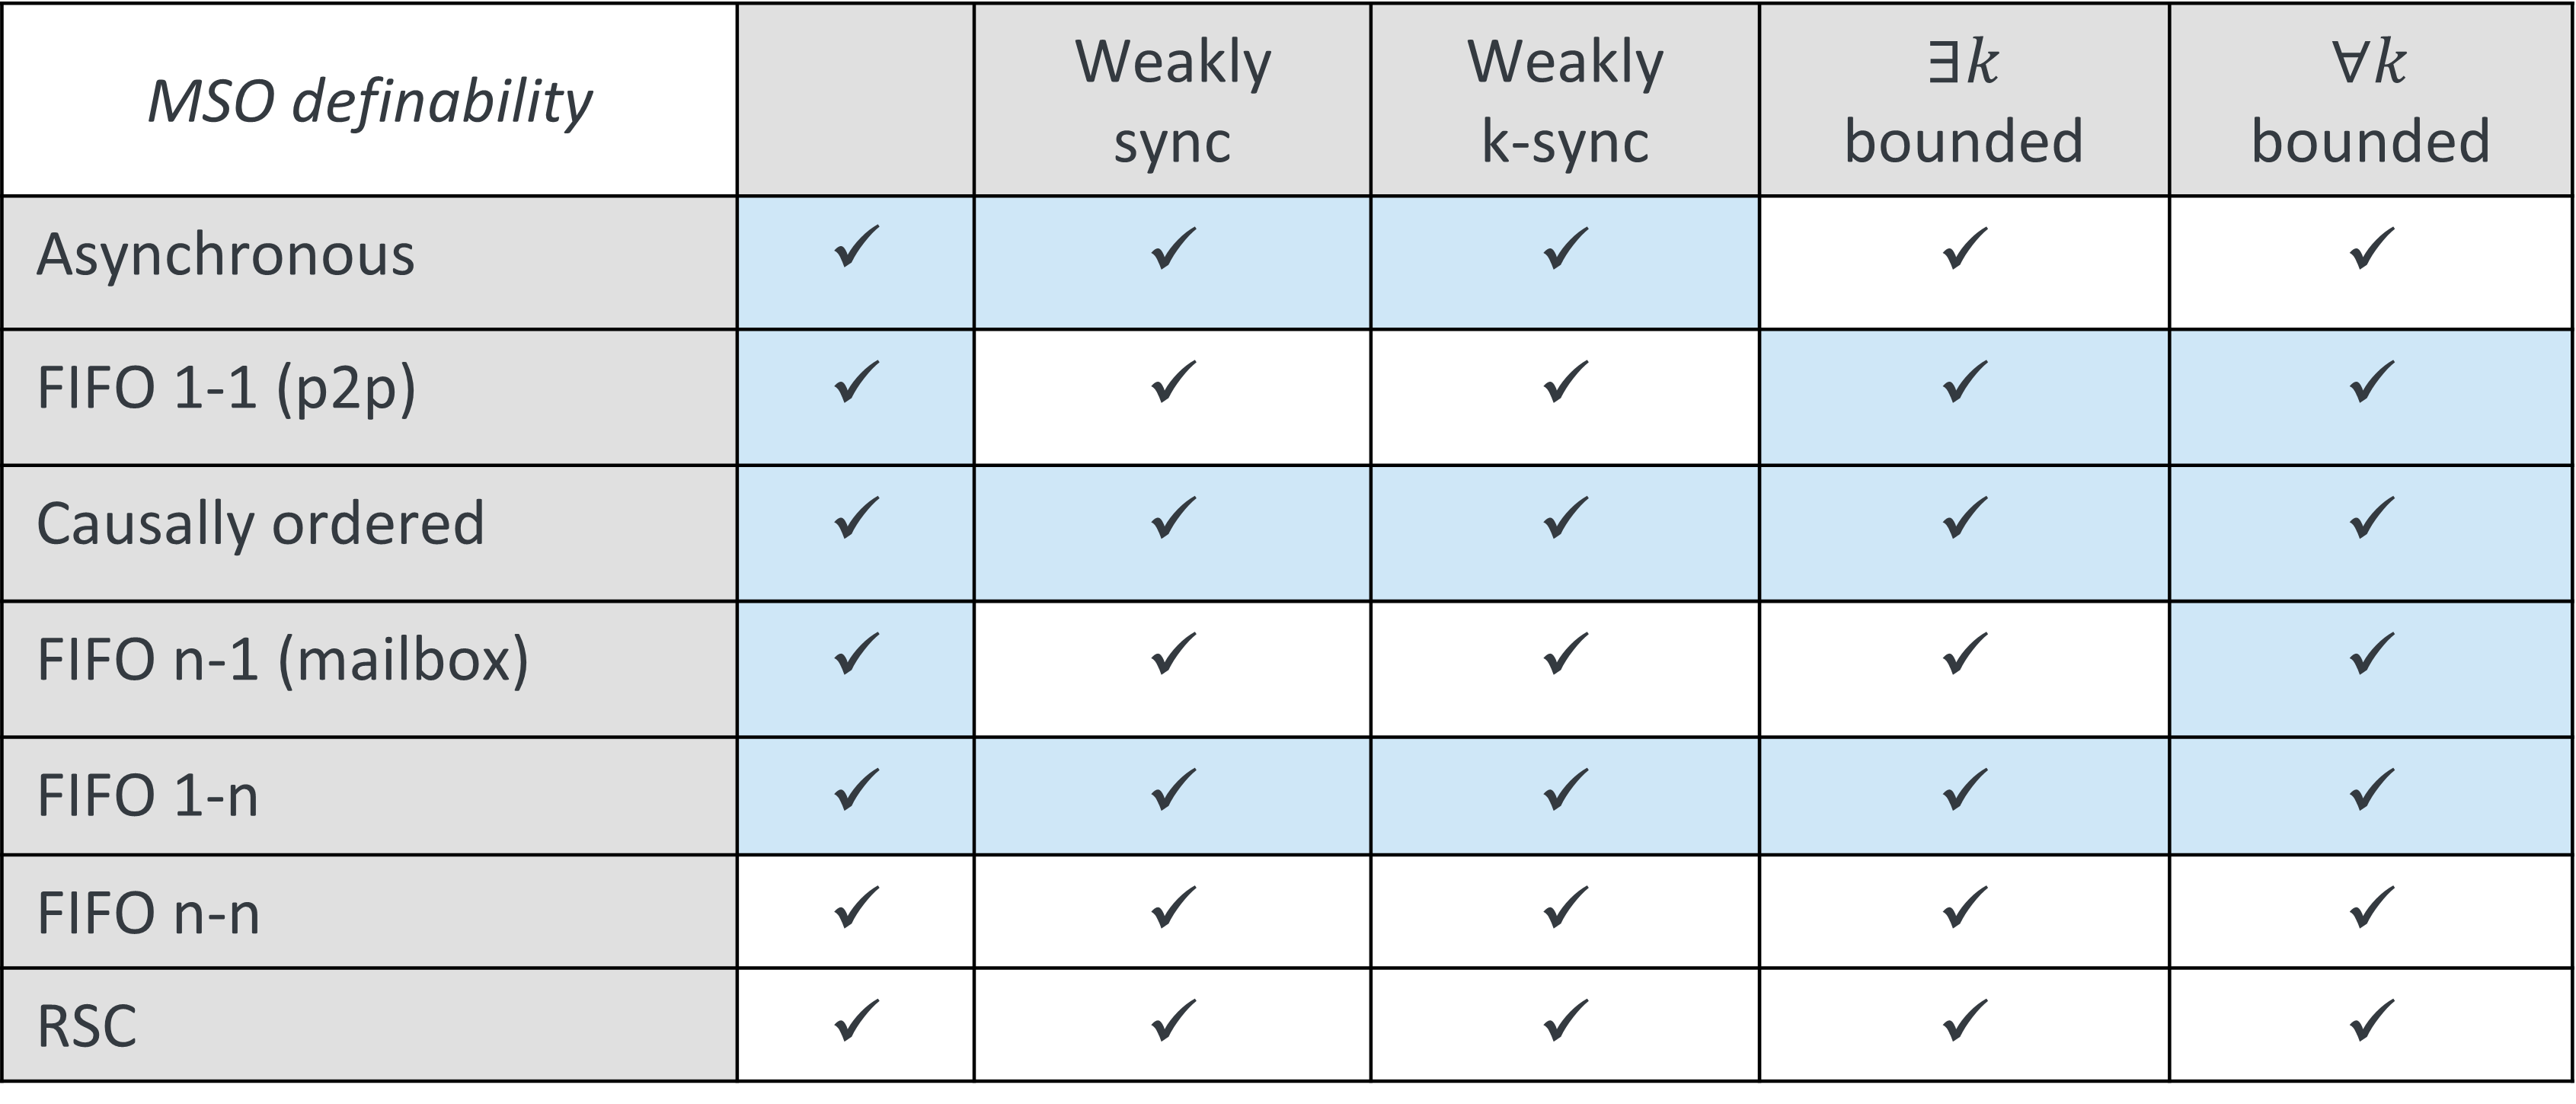
\includegraphics[width=10cm]{mso_def}
	\end{center}
\end{figure}

\begin{figure}[ht]
	\begin{center}
	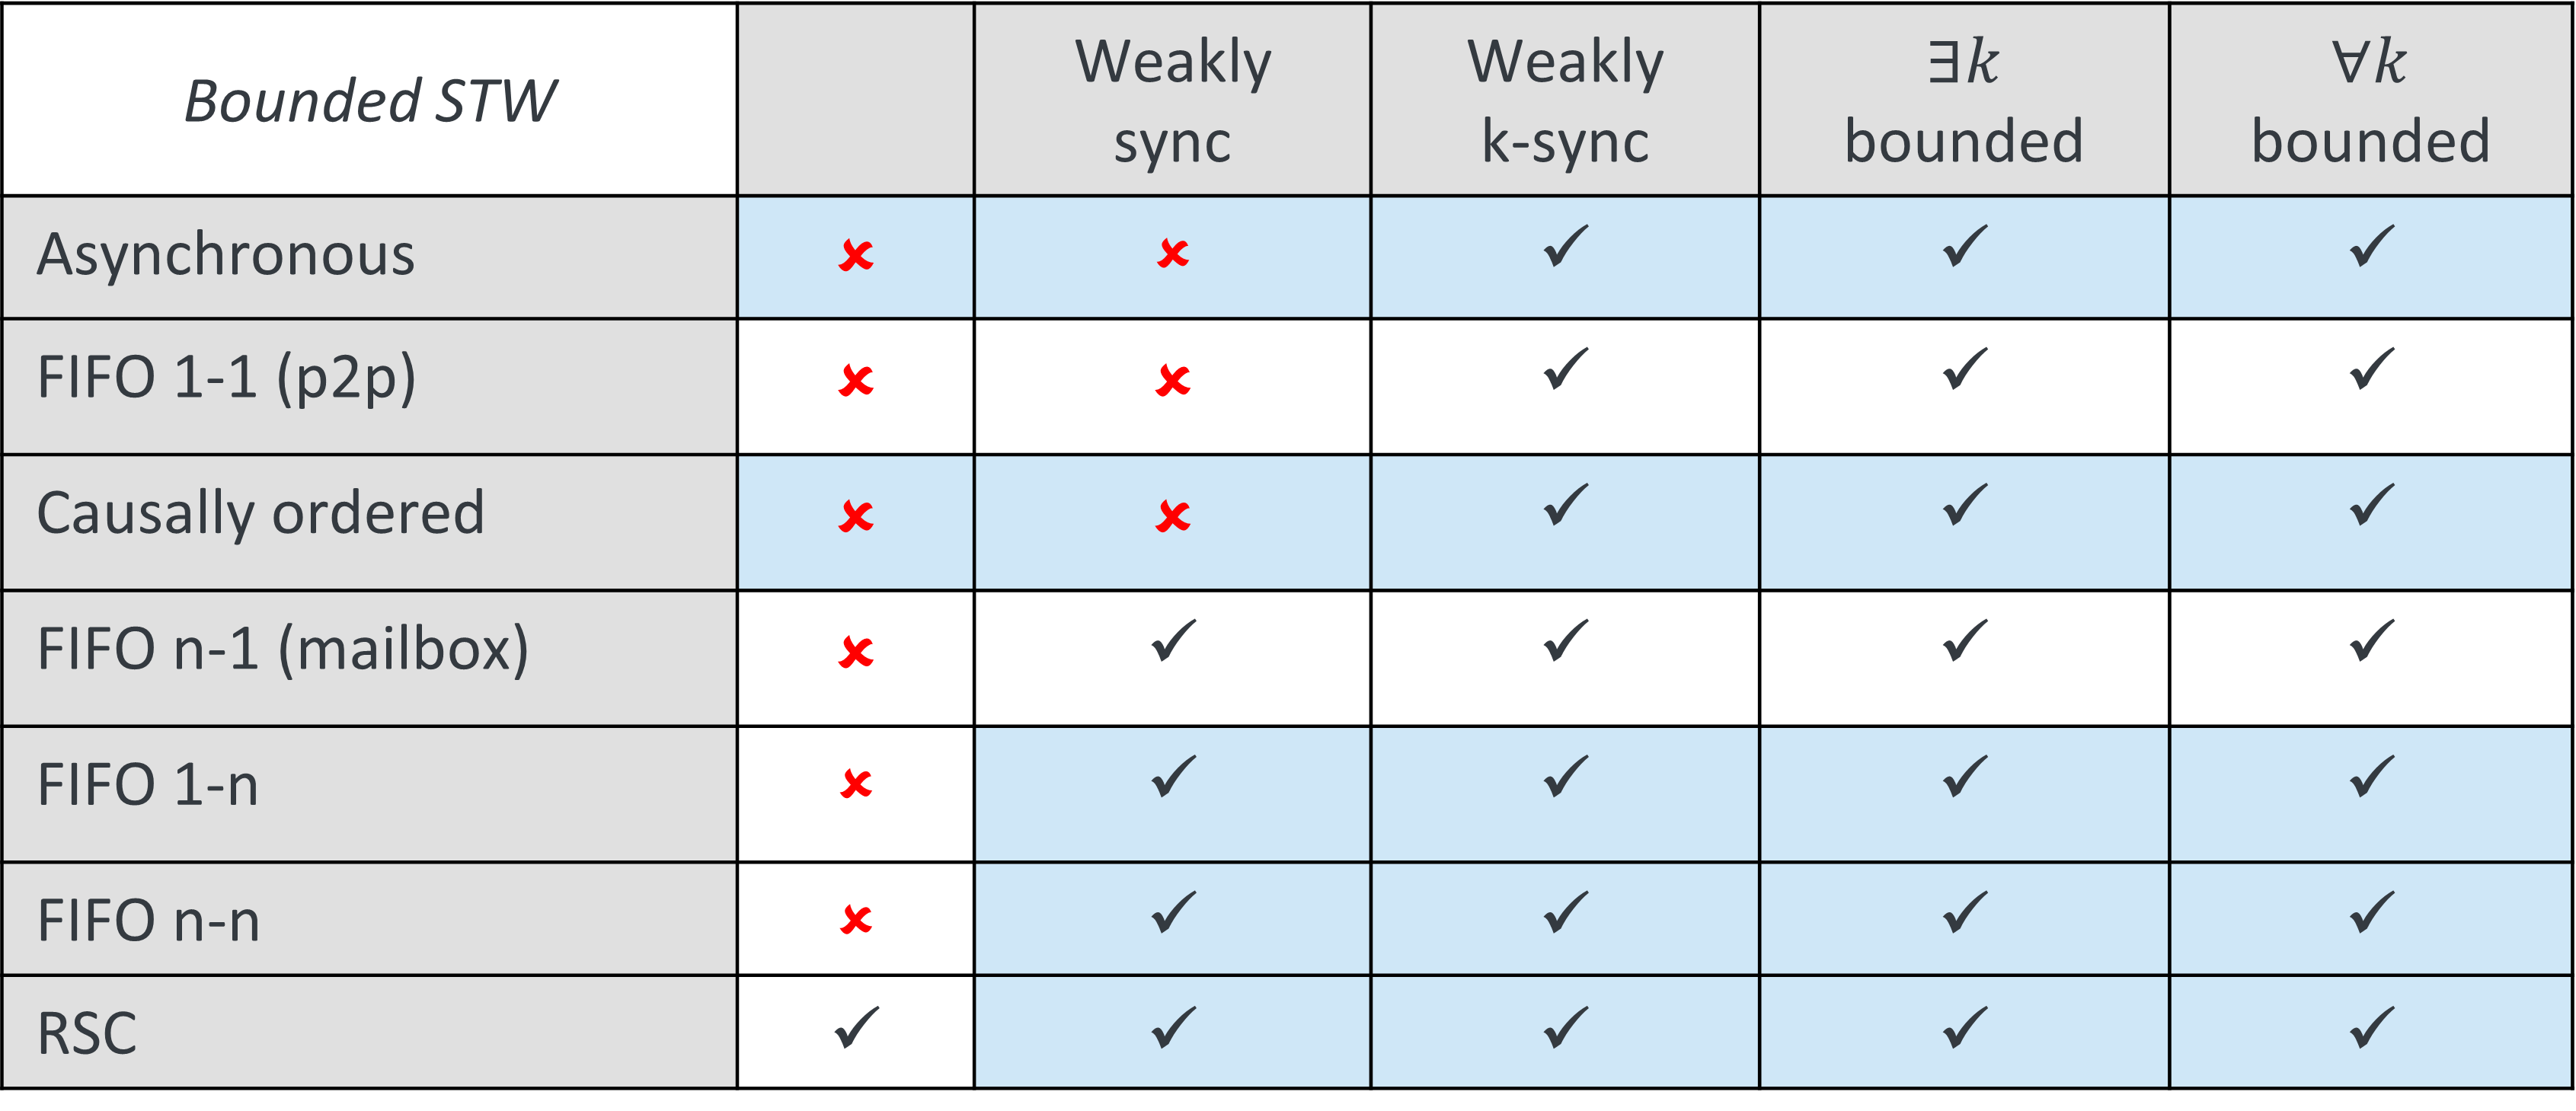
\includegraphics[width=10cm]{stw_bound}
	\end{center}
\end{figure}

In \cite{BolligFG21} the authors introduce a general framework based on MSO-logic and special treewidth (a graph property) that allows to derive decidability results for the \emph{synchronizability problem}. Roughly, the synchronizability problem consists in understanding whether all the behaviours/computations generated by a system have certain properties. The results in \cite{BolligFG21} hold for the $\oneone$ and the $\none$ communication models, which are referred to as p2p and mailbox, respectively. We show here that this framework can be effectively extended to all the 7 communication models that we considered.

\subsection{Special treewidth}

\emph{Special treewidth} \cite{Courcelle10},
is a graph measure that somehow indicates how close
a graph is to a tree (we may also use classical \emph{treewidth} instead).
This or similar measures are commonly employed in verification. For instance, treewidth and split-width have been used in \cite{MadhusudanP11} and, respectively, \cite{DBLP:conf/concur/CyriacGK12,AiswaryaGK14} to reason about graph behaviors generated by pushdown and queue systems.
%Here we apply it to reason about MSCs.
There are several ways to define the special treewidth of an MSC.
We adopt the following game-based definition from \cite{DBLP:journals/corr/abs-1904-06942}.

Adam and Eve play a turn based ``decomposition game'' on an MSC $\msc = (\Events, \procrel, \lhd, \lambda)$. $\msc$ is interpreted as a graph where nodes are the events and edges are represented by the $\procrel$ and the $\lhd$ relations.
Eve starts to play and does a move, which consists in the following steps:
\begin{enumerate}
	\item marking some events of $\msc$, resulting in the \emph{marked MSC fragment} $(M, U')$, where $U' \subseteq \Events$ is the subset of marked events,
	\item removing edges whose both endpoints are marked, in such a way that the resulting MSC is disconnected (i.e. there are at least two different connected components),
	\item splitting $(M, U)$ in $(M_1, U_1)$ and $(M_2, U_2)$ such that $M$ is the disjoint (unconnected) union of $M_1$ and $M_2$
	and marked nodes are inherited.
\end{enumerate}
Once Eve does her move, it is Adam's turn. Adam simply chooses one of the two marked MSC fragments, either $(M_1, U_1)$ or $(M_2, U_2)$. Now it is again Eve's turn, and she has to do a move on the marked MSC fragment that was chosen by Adam. The game continues in alternating turns between the two players until they reach a point where all the events on the current marked MSC fragment are marked.
For $k \in \N$, we say that the game is $k$-winning for Eve if she has a strategy that allows her, independently of Adam's moves, to end the game in a way that every marked MSC fragment visited during the game has at most $k+1$ marked events. The goal of Alice is to keep $k$ as low as possible.

% !TEX root = ../popl-paper.tex

\begin{figure}[t]
	\begin{center}
		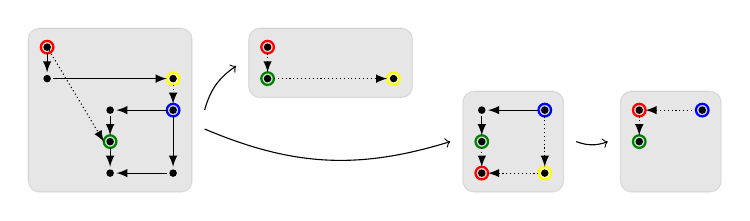
\begin{tikzpicture}[scale = .8]
			\begin{scope}
				\draw[gray,fill = gray, rounded corners, opacity=0.2] (-.3,.3) rectangle (2.3,-2.3);
				\draw[red, thick, fill = red!20] (0,0) circle (0.1);
				\draw[Green, thick, fill = Green!20] (1,-1.5) circle (0.1);
				\draw[Yellow, thick, fill = Yellow!20] (2,-.5) circle (0.1);
				\draw[blue, thick, fill = blue!20] (2,-1) circle (0.1);

				\draw[black, fill = black] (0,0) circle (.05);
				\draw[black, fill = black] (0,-.5) circle (.05);
				\draw[black, fill = black] (2,-.5) circle (.05);
				\draw[black, fill = black] (1,-1) circle (.05);
				\draw[black, fill = black] (2,-1) circle (.05);
				\draw[black, fill = black] (1,-1.5) circle (.05);
				\draw[black, fill = black] (1,-2) circle (.05);
				\draw[black, fill = black] (2,-2) circle (.05);

				\draw[>=latex, ->] (0,-.1) to (0, -.4);
				\draw[>=latex, ->,  densely dotted] (0,0) to (.9, -1.5);
				\draw[>=latex, ->] (.1,-.5) to (1.9, -.5);
				\draw[>=latex, ->,  densely dotted] (2,-.6) to (2, -.9);
				\draw[>=latex, ->] (1.9,-1) to (1.1, -1);
				\draw[>=latex, ->] (1,-1.1) to (1, -1.4);
				\draw[>=latex, ->] (1,-1.6) to (1, -1.9);
				\draw[>=latex, ->] (2,-1.1) to (2, -1.9);
				\draw[>=latex, ->] (1.9,-2) to (1.1, -2);

				\draw[->] (2.5,-1) to[bend left = 20] (3,-.3);
				\draw[->] (2.5,-1.3) to[bend right = 20] (6.4,-1.5);
				\draw[->] (8.4,-1.5) to[bend right = 20] (8.9,-1.5);


			\end{scope}
			\begin{scope}[shift = {(3.5,0)}]
				\draw[gray,fill = gray, rounded corners, opacity=0.2] (-.3,.3) rectangle (2.3,-.8);
				\draw[red, thick, fill = red!20] (0,0) circle (0.1);
				\draw[Green, thick, fill = Green!20] (0,-.5) circle (0.1);
				\draw[Yellow, thick, fill = Yellow!20] (2,-.5) circle (0.1);

				\draw[black, fill = black] (0,0) circle (.05);
				\draw[black, fill = black] (0,-.5) circle (.05);
				\draw[black, fill = black] (2,-.5) circle (.05);

				\draw[>=latex, ->, densely dotted	] (0,-.1) to (0, -.4);
				\draw[>=latex, ->, densely dotted	] (.1,-.5) to (1.9, -.5);
			\end{scope}
			\begin{scope}[shift = {(5.9,0)}]
				\draw[gray,fill = gray, rounded corners, opacity=0.2] (.7,-.7) rectangle (2.3,-2.3);
				\draw[red, thick, fill = red!20] (1,-2) circle (0.1);
				\draw[Green, thick, fill = Green!20] (1,-1.5) circle (0.1);
				\draw[Yellow, thick, fill = Yellow!20] (2,-2) circle (0.1);
				\draw[blue, thick, fill = blue!20] (2,-1) circle (0.1);

				\draw[black, fill = black] (1,-1) circle (.05);
				\draw[black, fill = black] (2,-1) circle (.05);
				\draw[black, fill = black] (1,-1.5) circle (.05);
				\draw[black, fill = black] (1,-2) circle (.05);
				\draw[black, fill = black] (2,-2) circle (.05);
				\draw[>=latex, ->] (1.9,-1) to (1.1, -1);
				\draw[>=latex, ->] (1,-1.1) to (1, -1.4);
				\draw[>=latex, ->,  densely dotted] (1,-1.6) to (1, -1.9);
				\draw[>=latex, ->,  densely dotted] (2,-1.1) to (2, -1.9);
				\draw[>=latex, ->,  densely dotted] (1.9,-2) to (1.1, -2);
			\end{scope}

			\begin{scope}[shift = {(8.4,0)}]
				\draw[gray,fill = gray, rounded corners, opacity=0.2] (.7,-.7) rectangle (2.3,-2.3);
				\draw[red, thick, fill = red!20] (1,-1) circle (0.1);
				\draw[Green, thick, fill = Green!20] (1,-1.5) circle (0.1);
				%\draw[Yellow, thick, fill = Yellow!20] (2,-2) circle (0.1);
				\draw[blue, thick, fill = blue!20] (2,-1) circle (0.1);

				\draw[black, fill = black] (1,-1) circle (.05);
				\draw[black, fill = black] (2,-1) circle (.05);
				\draw[black, fill = black] (1,-1.5) circle (.05);

				\draw[>=latex, ->,  densely dotted] (1.9,-1) to (1.1, -1);
				\draw[>=latex, ->,  densely dotted] (1,-1.1) to (1, -1.4);
				\end{scope}

		\end{tikzpicture}
	\end{center}
  \caption{Decomposition game for the MSC of Fig.~\ref{fig:pp_ex}. This is a 3-winning game for Eve.}
  \label{fig:stw-ex}
\end{figure}

\davide{Example of special treewidth}

\newcommand{\CS}[2]{\mathsf{CS}_{(#1,#2)}}
\newcommand{\MSO}[2]{\mathsf{MSO}_{(#1,#2)}}
\newcommand{\LCPDL}[2]{\mathsf{LCPDL}_{(#1,#2)}}
\newcommand{\MSCpm}[2]{\mathsf{MSC}_{(#1,#2)}}
\newcommand{\mbMSCpm}[2]{\mathsf{MSC}_{(#1,#2)}^{\mathsf{mb}}}


\begin{fact}[\cite{DBLP:journals/corr/abs-1904-06942}]
	The special treewidth of an MSC is the least $k$ such that
	the associated game is $k$-winning for Eve.
\end{fact}

The set of MSCs whose special treewidth is at most $k$ is denoted by $\stwMSCs{k}$.

\subsection{The synchronizability problem}

The synchronizability problem consists in understanding whether all the behaviours generated by a system, using some communication model, have a particular shape, i.e.  whether they are all included in a given set of MSCs $\Class$. Formally, the synchronizability problem is an inclusion problem, namely $\cL{\Sys} \subseteq \Class$, where $\comsymb \in \{$$\asy, $ $\oneone, $ $\co, $ $\none, $ $\onen, $ $\nn, $ $\rsc\}$. In \cite{BolligFG21} the authors show that, for $\comsymb = \oneone$ and $\comsymb = \none$, the synchronizability problem is decidable if $\Class$ is MSO-definable and special treewidth bounded (STW-bounded). In particular, among the classes $\Class$ that they considered, we will recall weakly synchronous, weakly k-synchronous, existentially $k$-bounded, and universally $k$-bounded MSCs. Fig.~\ref{} shows the results about decidability of the synchronizability problem for each of these classes and all 7 communication models. Theorem~\ref{thm:sync} is the main result that allows to derive the decidability of the synchronizability problem ($SP$ in the following).

\begin{theorem}\label{thm:sync}
	Fix finite sets $\Procs$ and $\Msg$.
	Let $\comsymb \in \{$$\asy, $ $\oneone, $ $\co, $ $\none, $ $\onen, $ $\nn, $ $\rsc\}$ and let $\Class \subseteq \MSCs$ be an MSO-definable and STW-bounded class (over $\Procs$ and $\Msg$).
	The following problem is decidable:
	given a communicating system $\System$, do we have $\cL{\System} \subseteq \Class$?
\end{theorem}

\davide{Maybe say why the synchronizability problem is important (if $\Class$ is STW-bounded and $L(S) \subseteq \Class$, then the model-checking problem for $S$ becomes decidable because it recuces to bounded model-checking)... but we should also talk about what is bounded model-checking}


%%%%%% COPY-PASTE from report

% \subsection{Semantics of causal ordering}

% \newcommand{\buffers}{\vv{\text{Buf}}}
% \newcommand{\clocks}{\vv{\text{Vec}}}
% \begin{definition}
% 	Given a system $\System = (Loc_p, \delta_p, \ell^0_p)_{p\in\procSet}$ with $n$ processes, a \emph{configuration} is a tuple $(\vv{\ell},\buffers,\clocks)$, where $\vv{\ell}=(\ell_p)_{p \in \procSet}$ represents the global state of the system, $\buffers=(b_p)_{p \in \procSet}$ is a vector of buffers, with each $b_p \in \Msg^*$ representing the content of the buffer of process $p$, and $\clocks=(v_p)_{p \in \procSet}$ is a vector of Mattern-Fidge logical clocks, where each $v_p = (time_i)_{i \in \procSet}$ represents the content of the logical vector clock of process $p$.
% \end{definition}

\subsection{Weakly synchronous MSCs}

We first introduce the class of weakly synchronous MSCs. This is a generalization of synchronous MSCs studied earlier, in \cite{DBLP:conf/cav/BouajjaniEJQ18, DBLP:conf/fossacs/GiustoLL20}. We say an MSC is weakly synchronous if it is breakable into \emph{exchanges}, where an exchange is an MSC that allows one to schedule all sends before all receives. Before giving the formal definition, we need the notion of \emph{concatenation} of MSCs.

\davidequestion{The following definition works for p2p, but it should be changed for asynchronous (remove the condition on unmatched messages.)}

Let $\msc_1 = (\Events_1,\procrel_1,\lhd_1,\lambda_1)$ and
$\msc_2 = (\Events_2,\procrel_2,\lhd_2,\lambda_2)$ be two MSCs.
Their \emph{concatenation} $\msc_1 \cdot \msc_2 = (\Events,\procrel,\lhd,\lambda)$ is defined if, for all $(p,q) \in \Ch$,
$e_1 \in \Unm{\msc_1}$, and
$e_2 \in \Events_2$ such that $\lambda(e_1) \in \pqsAct{p}{q}$
and $\lambda(e_2) \in \pqsAct{p}{q}$,
we have $e_2 \in \Unm{\msc_2}$.
As expected, $\Events$ is the disjoint union of $\Events_1$ and $\Events_2$,
${\lhd}  = {\lhd_1} \cup {\lhd_2}$, $\lambda$ is the ``union'' of $\lambda_1$
and $\lambda_2$, and ${\procrel} = {\procrel_1} \cup {\procrel_2} \cup R$.
Here, $R$ contains, for all $p \in \Procs$ such that $(\Events_1)_p$ and
$(\Events_2)_p$ are non-empty, the pair $(e_1,e_2)$ where $e_1$ is the
maximal $p$-event in $M_1$ and $e_2$ is the minimal $p$-event in $M_2$.
Note that $\msc_1 \cdot \msc_2$ is indeed an MSC and that
concatenation is associative.

\begin{definition}[exchange]\label{def:weak-synchr}
Let $\msc = (\Events,\procrel,\lhd,\lambda)$ be an MSC.
We say that $\msc$ is an \emph{exchange} if
$\SendEv{\msc}$ is
a ${\le_\msc}$-downward-closed set.
\end{definition}

In other words, an exchange is an MSC $\msc$ where no send event depends on another receive event. If that is the case, we can find a linearization for $\msc$ where all the send events are executed before the receive events.

\begin{definition}[weakly synchronous]\label{def:weaksync-new}
	We say that $\msc \in \MSCs$ is
	\emph{weakly synchronous} if it is of the form
	$\msc = \msc_1 \cdot \ldots \cdot \msc_n$
	such that every $\msc_i$ is an exchange.
\end{definition}

\noindent
\begin{minipage}[c]{10.5cm}
	\begin{example}\label{example:msc_W}
		Consider the MSC $\mscW$ in Fig.~\ref{fig:msc_W}. It is is weakly synchronous. Indeed, $\amessage_1$, $\amessage_2$, and $\amessage_5$ are independent and can be put alone in an exchange. Repetitions of $\amessage_3$ and $\amessage_4$ are interlaced, but they constitute an exchange, as we can do all sends and then all receptions.
	\end{example}
\end{minipage}
\hfill
\begin{minipage}[c]{3cm}
	\begin{center}
	  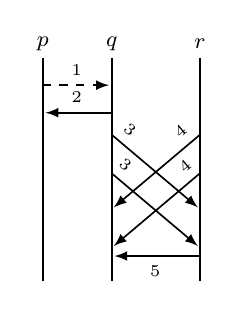
\begin{tikzpicture}[>=stealth,node distance=3.4cm,shorten >=1pt,
	  every state/.style={text=black, scale =0.6}, semithick,
		font={\fontsize{8pt}{12}\selectfont}]

	\begin{scope}[shift = {(8,0.75)}, scale = 0.7]
	  %MACHINES
	  \draw (0,1.25) node{$q$} ;
	  \draw (1.6,1.25) node{$r$} ;
	  \draw (-1.25,1.25) node{$p$} ;
	  \draw (0,1) -- (0,-3.1) ;
	  \draw (1.6,1) -- (1.6,-3.1);
	  \draw (-1.25,1) -- (-1.25,-3.1);

	  %MESSAGES
	  \draw[>=latex,->, dashed] (-1.25, 0.5) -- (0, 0.5) node[ above, midway] {$\amessage_1$};
	  \draw[>=latex,->] (0, 0) -- (-1.25, 0) node[ above, midway] {$\amessage_2$};


	  \draw[>=latex,->] (0, -0.4) -- (1.6, -1.75) node[pos=0.1, sloped, above] {$\amessage_3$};
	  \draw[>=latex,->] (0, -1.1) -- (1.6, -2.45) node[pos=0.05, sloped, above] {$\amessage_3$}; %{$\amessage_1'$};
	  %\draw[>=latex,->, dashed] (0, -2.5) -- (1.25, -3.25) node[pos=0.55, sloped, above] {$\amessage_1''$};

	  \draw[>=latex,->] (1.6, -0.4) -- (0, -1.75) node[pos=0.1, sloped, above] {$\amessage_4$};
	  \draw[>=latex,->] (1.6, -1.1) -- (0, -2.45) node[pos=0.05, sloped, above] {$\amessage_4$}; %{$\amessage_2'$};
	  %\node[rotate = 90, left]at (1.13, -0.65) {$\cdots$};
	  %\node[rotate = -90, right]at (0.1, -0.65) {$\cdots$};

	  \draw[>=latex,->] (1.6, -2.6) -- (0, -2.6) node[ below, midway] {$\amessage_5$};


	\end{scope}

	\end{tikzpicture}
	\captionof{figure}{MSC $\mscW$}
	\label{fig:msc_W}
	\end{center}
\end{minipage}

In \cite{BolligFG21} it is shown that, for the class of weakly synchronous MSCs, $SP$ is undecidable for $\comsymb = \oneone$, but decidable for $\comsymb = \oneone$.

Here we address the decidability of $SP$ for the class of weakly synchronous MSCs, considering also other communication models (these results are summarized in the second column of Fig.\ref{}). We now show that $SP$ is undecidable also for causally ordered communication.

\begin{proposition}\label{thm:co-weak-sync}
	The following problem is undecidable:
	Given finite sets $\Procs$ and $\Msg$ as well as a communicating system $\System$,
	is every MSC in $\coL{\System}$ weakly synchronous?
\end{proposition}
\begin{proof}
	The proof is essentially identical to that given in \cite{BolligFG21} for the $\oneone$ case. We do the same reduction from the Post correspondence problem. The original proof considered a $\oneone$ system $\System$ with four machines (P1, P2, V1, V2), where we have unidirectional communication channels from provers (P1 and P2) to verifiers (V1 and V2). In particular notice that all the possible behaviours of $\System$ are causally ordered, i.e. $\ppL{\System} \subseteq \coMSCs$; according to how we built our system $\System$, it is impossible to have a pair of causally-related send events of P1 and P2\footnote{There is no channel between P1 and P2, and we only have unidirectional communication channels from provers to verifiers; it is impossible to have a causal path between two send events of P1 and P2.}, which implies that causal ordering is already ensured by any possible $\oneone$ behaviour of $\System$. The rest of the proof is identical to the $\oneone$ case.
\end{proof}

The hierarchy in Fig.~\ref{fig:msc_hierarchy_full} and the MSO formulas given in Section~\ref{} allow us to derive the decidability of $SP$ for the remaining communcation models.

\begin{proposition}\label{thm:weak-sync}
	Let $\comsymb \in \{$$\onen, $ $\nn, $ $\rsc\}$.
	The following problem is decidable:
	given finite sets $\Procs$ and $\Msg$ as well as a communicating system $\System$,
	is every MSC in $\cL{\System}$ weakly synchronous?
\end{proposition}
\begin{proof}
	We will consider $\comsymb = \onen$; the proof for the other communication models follows the same steps. We would like to know if every MSC in $\onenL{\System}$ is in the class of weakly synchronous MSCs. Since every MSC in $\onenL{\System}$ is a $\onen$ MSC, we can equivalently restrict the problem to the class of weakly synchronous MSCs that are also $\onen$ MSCs. Let $\Class$ be the class of $\onen$ weakly synchronous MSCs; we show that $\Class$ is MSO-definable and STW-bounded, which implies the decidability of $SP$ for Theorem~\ref{thm:sync}. The class of weakly synchronous MSCs was shown to be MSO-definable in \cite{BolligFG21}; to be precise, their characterization is for $\oneone$ weakly synchronous MSCs (since their definition of MSC is equivalent to our definition of $\oneone$ MSC), but it also works for (asynchronous) weakly synchronous MSCs. We showed in Section~\ref{} that $\onenMSCs$ is MSO-definable; it follows that the class of $\onen$ weakly synchronous MSCs is also MSO-definable (we just take the conjuction of the the two formulas). The class of $\none$ weakly synchronous MSCs was shown to be STW-bounded in \cite{BolligFG21}, and since $\onenMSCs \subset \mbMSCs$, we also have that the class of $\none$ weakly synchronous MSCs has a bounded special treewidth. The claim follows from Theorem~\ref{thm:sync}.
\end{proof}

\subsection{Weakly \texorpdfstring{$k$}{k}-synchronous MSCs}

The undecidability result for some of the communication models motivates the study of other classes. Here we present weakly $k$-synchronous MSCs (\cite{BolligFG21}), which are a variant of weakly synchronous MSCs where the number of messages sent per exchange is at most $k$.

\begin{definition}[$k$-exchange]\label{def:weak-k-synchr}
Let $\msc = (\Events,\procrel,\lhd,\lambda)$ be an MSC
and $k \in \N$.
We call $\msc$ a $k$-\emph{exchange} if
$\msc$ is an exchange and $|\SendEv{\msc}| \le k$.
\end{definition}

\begin{definition}[weakly $k$-synchronous]\label{def:weaksync}
Let $k \in \N$.
We say that $\msc \in \MSCs$ is
weakly $k$-synchronous if it is of the form
$\msc = \msc_1 \cdot \ldots \cdot \msc_n$
such that every $\msc_i$ is a $k$-exchange.
\end{definition}

\noindent
\begin{minipage}[c]{10.5cm}
	\begin{example}
	MSC $\mscweakSexist$ in Fig.~\ref{fig:msc_weak_S_exist} is weakly $1$-synchronous, as it can be
	decomposed  into three \kE{1}s (the decomposition is depicted by the
	horizontal dashed lines). We remark that $\mscweakSexist \in
	\mbMSCs$. Note that there is a p2p linearization that respects the decomposition.
	On the other hand, a mailbox linearization needs to reorganize actions from different MSCs: the sending of
	$\msg_3$ needs to be done before the sending of $\msg_1$. Note that $\mscweakuniver$ in
	Fig.~\ref{fig:msc_weak_univer} is also weakly $1$-synchronous.
	\end{example}
\end{minipage}
	\hfill
\begin{minipage}[c]{3cm}
\begin{center}

	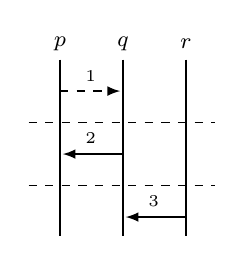
\begin{tikzpicture}[>=stealth,node distance=3.4cm,shorten >=1pt,
		every state/.style={text=black, scale =0.7}, semithick,
		font={\fontsize{8pt}{12}\selectfont}, scale = 0.8]

	  %MACHINES
	  \draw (0,0) node{$p$} ;
	  \draw (1,0) node{$q$} ;
	  \draw (2,0) node{$r$} ;
	  \draw (0,-0.25) -- (0,-3.1) ;
	  \draw (1,-0.25) -- (1,-3.1);
	  \draw (2, -0.25) -- (2, -3.1) ;
	  %MESSAGES
	  \draw[>=latex,->, dashed] (0,-0.75) -- (1, -0.75) node[midway,above]{$\amessage_1$};

	  \draw[>=latex,->] (1, -1.75) -- (0, -1.75) node[midway, above] {$\amessage_2$};
	  %\draw (0.5,-1.7) node{$\cdots$};
	  %\draw[>=latex,->] (1, -2.25) -- (0, -2.25) node[midway, above] {$\amessage_2$};

	  \draw[>=latex,->] (2,-2.75) -- (1,-2.75) node[midway, above] {$\amessage_3$};
	%\end{scope}
	  \draw[dashed] (-0.5,-1.25) -- (2.5,-1.25) ;
	  \draw[dashed] (-0.5,-2.25) -- (2.5,-2.25) ;


	\end{tikzpicture}
	\captionof{figure}{MSC $\mscweakSexist$}
	\label{fig:msc_weak_S_exist}

\end{center}
\end{minipage}

As for weakly synchronous MSCs, the class of weakly $k$-synchronous MSCs was already shown to be MSO-definable and STW-bounded in \cite{BolligFG21}, and these results still hold even for our definition of MSC. A direct application of Theorem~\ref{thm:sync} shows that, for weakly $k$-synchronous MSCs, $SP$ is decidable for all communication models.

\begin{proposition}\label{thm:weak-k-sync}
	Let $\comsymb \in \{$$\asy, $ $\oneone, $ $\co, $ $\none, $ $\onen, $ $\nn, $ $\rsc\}$.
	The following problem is decidable:
	given finite sets $\Procs$ and $\Msg$ as well as a communicating system $\System$,
	is every MSC in $\cL{\System}$ weakly $k$-synchronous?
\end{proposition}
\begin{proof}
	The class $\Class$ of weakly $k$-synchronous MSCs is MSO-definable and STW-bounded. $SP$ is decidable for Theorem~\ref{thm:sync}.
\end{proof}

\davide{End of edited section}

\subsection{Weakly synchronous causally ordered MSCs}

Corollary~\ref{cor:weak-sync-lcpdl} can  be extended to $\comsymb = \cosymb$.

\begin{proposition}\label{cor:co-weak-sync-mso}
The set of weakly synchronous \emph{causally ordered} MSCs is MSO-definable.
\end{proposition}
\begin{proof}
Both the sets of weakly synchronous MSCs and of causally ordered MSCs are MSO-definable, as shown by Corollary~\ref{cor:weak-sync-lcpdl} and Proposition~\ref{prop:co_mso}. Recall that any LCPDL-definable property is also MSO-definable. It suffices to take the conjuction of the two respective MSO formulas.
\end{proof}

\begin{theorem}\label{thm:co-weak-sync}
The following problem is undecidable:
Given finite sets $\Procs$ and $\Msg$ as well as a communicating system $\System$,
is every MSC in $\coL{\System}$ weakly synchronous?
\end{theorem}
\begin{proof}
The proof is essentially identical to the \pp case. We do the same reduction from the Post correspondence problem. Recall from the proof of Theorem~\ref{thm:p2p-weak-sync} that we consider a system $\System$ with four machines (P1, P2, V1, V2), where we have unidirectional communication channels from provers to verifiers. In particular notice that all the possible behaviours of $\System$ are causally ordered, i.e. $\ppL{\System} \subseteq \coMSCs$; according to how we built our system $\System$, it is impossible to have a pair of causally-related send events of P1 and P2\footnote{There is no channel between P1 and P2, and we only have unidirectional communication channels from provers to verifiers; it is impossible to have a causal path between two send events of P1 and P2.}, which implies that causal ordering is already ensured by any possible \pp behaviour of $\System$. The rest of the proof is identical to the \pp case.
\end{proof}

\begin{corollary}
The set of weakly synchronous causally ordered MSCs has unbounded special treewidth.
\end{corollary}
\begin{proof}
Suppose that the set of weakly synchronous causally ordered MSCs is STW-bounded. By Proposition \ref{cor:co-weak-sync-mso} and Theorem~\ref{thm:sync_co}, we have that the syncronicity problem for the class of weakly synchronous causally ordered MSCs would be decidable. This is a contradiction, since Theorem~\ref{thm:co-weak-sync} states that this problem is undecidable.
\end{proof}

\subsection{Weakly \texorpdfstring{$k$}{k}-synchronous causally ordered MSCs}

\begin{proposition}\label{prop:co-weak-k-sync-mso}
The set of weakly \emph{k}-synchronous causally ordered MSCs is MSO-definable.
\end{proposition}
\begin{proof}
Both the sets of weakly \emph{k}-synchronous MSCs and of causally ordered MSCs are MSO-definable, as shown by Proposition~\ref{prop:weak-logic-bounded} and Proposition~\ref{prop:co_mso}. It suffices to take the conjuction of the two respective MSO formulas.
\end{proof}

% Note that every causally ordered \emph{k}-synchronous MSC is also a  $\ppsymb$ \emph{k}-synchronous MSC.
Theorem~\ref{thm:sync} can be easily extended to $\comsymb = \cosymb$.

\begin{theorem}\label{thm:co-weak-k-sync}
For $\comsymb \in \{\ppsymb, \mbsymb,\cosymb\}$, the following problem is decidable:
Given finite sets $\Procs$ and $\Msg$, a communicating system $\System$, and $k \in \N$,
is every MSC in $\cL{\System}$ weakly $k$-synchronous?
\end{theorem}
\begin{proof}
By Proposition~\ref{prop:co-weak-k-sync-mso} and Proposition~\ref{prop:kweakstw} we have that the class of causally ordered \emph{k}-synchronous MSCs is MSO-definable and STW-bounded\footnote{Note that Proposition~\ref{prop:kweakstw} is independent from the type of communication.}. Theorem~\ref{thm:sync_co} ends the proof.
\end{proof}

\subsection{Existentially \texorpdfstring{$k$}{k} causally ordered bounded MSCs}

\begin{definition}
Let $\msc = (\Events,\procrel,\lhd,\lambda) \in \MSCs$ and $k \in \N$.
A linearization $\linrel$ of $\msc$ is called
$k$-\emph{bounded} if, for all $e \in \Matched{\msc}$, with $\lambda(e) = \sact{p}{q}{\msg}$, we have
\[
\sametype{e}{\pqsAct{p}{q}}{\linrel} - \sametype{e}{\pqrAct{p}{q}}{\linrel} \le k.
\]
\end{definition}
\noindent Recall that $\sametype{e}{\pqsAct{p}{q}}{\linrel}$ denotes the number of send events from $p$ to $q$ that occured before $e$, according to $\linrel$.

\begin{definition}\label{def:ex_k_pp_bounded}
	An MSC is said to be \emph{existentially \pp bounded} ($\exists k$-$\pp$-bounded) if it has a $k$-bounded linearization.
\end{definition}

\begin{definition}\label{def:ex_k_co_bounded}
An MSC is said to be \emph{existentially $k$ causally ordered bounded} ($\exists k$-$\cosymb$-bounded) if it is causally ordered and it has a $k$-bounded linearization.
\end{definition}

Note that every existentially $k$ causally ordered bounded MSC is an existentially $k$-\pp-bounded MSC.

\begin{proposition}\label{prop:ek-co-bounded-mso-stw}
For all $k \in \N$, the set of $\exists k$-$\cosymb$-bounded MSCs is MSO-definable and STW-bounded.
\end{proposition}
\begin{proof}
Let $\ppEk$ and $\coEk$ be the set of existentially $k$-\pp-bounded MSCs and the set of existentially $k$ causally ordered bounded MSCs, respectively. $\ppEk$ was shown to be both MSO-definable (in \cite{DBLP:journals/iandc/LohreyM04}) and STW-bounded (in \cite[Proposition 5.4, page 163]{DBLP:journals/corr/abs-1904-06942}). $\coEk$ also has to be STW-bounded, since we have $\coEk \subseteq \ppEk$. Note that, by definition, $\coEk = \ppEk\, \cap\, \coMSCs$. Since both $\ppEk$ and $\coMSCs$ can be defined by an MSO formula, the latter according to Proposition~\ref{prop:co_mso}, $\coEk$ is also MSO-definable\footnote{Suppose $\varphi_{\exists k\text{-}\pp\text{-}b}$ is the MSO formula for $\ppEk$, and $\coformula$ is the MSO formula for $\coMSCs$. Then, $\coEk$ is defined by $\varphi_{\exists k\text{-}\cosymb\text{-}b} = \varphi_{\exists k\text{-}\pp\text{-}b} \wedge \coformula$}.
\end{proof}

\begin{theorem}\label{thm:sync_ek_co_bounded}
	The following problem is decidable: Given finite sets $\Procs$ and $\Msg$, a communicating system $\System$, and $k \in \N$, is every MSC in $\coL{\System}$ $\exists k$-$\cosymb$-bounded?
\end{theorem}
\begin{proof}
	Directly follows from \ref{prop:ek-co-bounded-mso-stw} and \ref{thm:sync_co}.
\end{proof}

\subsection{Existentially bounded MSCs}

\davidequestion{Should we say for all sends, also unmatched? Shouldn't it be $<$ instead of $\le$?}
\begin{definition}\label{def:lin_k_bounded}
	Let $\msc = (\Events,\procrel,\lhd,\lambda) \in \MSCs$ and $k \in \N$.
	A linearization $\linrel$ of $\msc$ is called
	$k$-\emph{bounded} if, for all $e \in \Matched{\msc}$, with $\lambda(e) = \sact{p}{q}{\msg}$, we have
	\[
	\sametype{e}{\pqsAct{p}{q}}{\linrel} - \sametype{e}{\pqrAct{p}{q}}{\linrel} \le k.
	\]
\end{definition}
\noindent Recall that $\sametype{e}{\pqsAct{p}{q}}{\linrel}$ denotes the number of send events from $p$ to $q$ that occured before $e$, according to $\linrel$. Intuitively, a linearization is $k$-bounded if, at any moment in time, there are no more than $k$ messages in any channel.

\begin{definition}[Existentially bounded MSC]\label{def:ek_bounded_msc}
	Let $\msc = (\Events, \rightarrow, \lhd, \lambda) \in \asMSCs$ and $k \in \mathbb{N}$. We call $\msc$ \emph{existentially $k$-bounded} if it has a $k$-bounded linearization.
\end{definition}
Let $\asEk$ be the set of existentially $k$-bounded MSCs, for a given $k \in \N$.
\begin{definition}
	An MSC $\msc$ is \emph{\pp existentially $k$-bounded} (\pp-$\exists k$-bounded) if it is a \pp MSC and it is also existentially $k$-bounded.
\end{definition}
\begin{definition}
	An MSC $\msc$ is \emph{causally orderered existentially $k$-bounded} ($\cosymb$-$\exists k$-bounded) if it is a causally ordered MSC and it is also existentially $k$-bounded.
\end{definition}
When moving on to mailbox MSCs, the definition of mailbox existentially $k$-bounded MSC should require that there exists a $k$-bounded linearization that is also a mailbox linearization, not just any linearization. Recall that an MSC is a mailbox MSC if it has at least one mailbox linearization, which represents a sequence of events that can be executed by a mailbox system. Following this intuition, we want one of these mailbox linearizations to be $k$-bounded, because \emph{non}-mailbox linearizations cannot be executed by a mailbox system.
\begin{definition}
	An MSC $\msc$ is \emph{mailbox existentially $k$-bounded} (mb-$\exists k$-bounded) if it is a mailbox MSC and it has a $k$-bounded mailbox linearization.
\end{definition}
\davide{This paragraph depends on how we choose to formally define the mailbox communication model... we could go for a (i) single incoming channel, or (ii) just an enforcing of the delivery of messages by the transport layer.}
It should be noted that, for a $k$-bounded mailbox linearization, it is not necessarily true that at any time we have at most $k$ messages in each channel. Recall that in the mailbox communication architecture every process has a single incoming channel, but the Definition~\ref{def:lin_k_bounded} of $k$-bounded linearization considers the number of pending messages between each pair $(p,q)$ of processes. Let $n$ be the number of processes. We can say that, for a $k$-bounded mailbox linearization, we have at most $k(n-1)$ messages in each channel at any moment (because each process can have at most $k$ pending messages coming from any of the other $n-1$ processes).
\davide{An example would be nice.}

\begin{definition}
	An MSC $\msc$ is \emph{$\onen$ existentially $k$-bounded} (1n-$\exists k$-bounded) if it is a $\onen$ MSC and it has a $k$-bounded $\onen$ linearization.
\end{definition}

\subsubsection{MSO-definability}

In this section, we will investigate the MSO-definability of all the variants of $\exists k$-bounded MSCs that we introduced, starting from the asynchronous $\exists k$-bounded MSCs.

% \begin{proposition}\label{prop:as_ex_k_b_alt}
% 	An asynchronous MSC $\msc$ is existentially $k$-bounded if and only if both the following hold:
% 	\begin{enumerate}
% 		\item We cannot find $k+1$ send events $s_1, \dots, s_{k+1}$ from a process $p$ to a process $q$, such that $s_1 \procrel^+ \dots \procrel^+ s_{k+1}$, $s_{k+1}$ is matched, i.e. $s_{k+1} \lhd r_{k+1}$, and $r_{k+1}$ happens before all the receive events for the matched send events between $s_1$ and $s_k$.
%   		\item We cannot find $k$ unmatched send events $s_1, \dots, s_{k}$ from a process $p$ to a process $q$, such that $s_1 \procrel^+ \dots \procrel^+ s_{k}$.
% 	\end{enumerate}
% \end{proposition}
% \begin{proof}
% 	\davide{Missing proof.}
% 	Let $\msc$ be an asynchronous MSC.\newline
% 	($\Rightarrow$) Suppose $\msc$ is $\exists k$-bounded. We prove the contrapositive, i.e. if either (1) or (2) do not hold, $\msc$ is not $\exists k$-bounded. Suppose (1) does not hold, so we are able to find a sequence $s_1, \dots, s_{k+1}$ with the described properties. $\msc$ is clearly not $\exists k$-bounded, since we must execute all the sends up to $s_{k+1}$ ($k+1$ sends in total) before being able to execute $r_{k+1}$, which happens before the other receive events. \newline
% 	($\Leftarrow$) Suppose both (1) and (2) hold for $\msc$.
% \end{proof}

% Using Proposition~\ref{prop:as_ex_k_b_alt}, we can give an MSO formula for the asynchronous existentially $k$-bounded MSCs.
% \[
% 	\psi_{asy-\exists k} = \psi_1 \vee \psi_2
% \]
% where $\psi_1$ and $\psi_2$ are
% \[
% 	\psi_1 = \nexists s_1 \dots \nexists s_{k+1}. \left(
% 	\begin{array}{llr}
% 		& allDistSend\_p\_q(k+1) & \quad\wedge\quad \\
% 		& s_1 \procrel^+ \dots \procrel^+ s_k & \quad\wedge\quad \\
% 		& \exists r_{k+1}. \left(
% 			\begin{array}{rl}
% 				& s_{k+1} \lhd r_{k+1} \quad\wedge\quad \\
% 				& \bigwedge_{s \in s_1 \dots s_k}
% 				(\exists r.s \lhd r \implies r_{k+1} \procrel^\ast r) \\
% 			\end{array}
% 		\right) &\\
% 	\end{array}
% 	\right)
% \]
% \[
% 	\psi_2 = \nexists s_1 \dots \nexists s_{k}.
% 		allDistSend\_p\_q(k) \;\wedge\;
% 		s_1 \procrel^+ \dots \procrel^+ s_k \;\wedge\;
% 		\bigwedge_{s \in s_1 \dots s_k} \neg \mathit{matched}(s)
% \]
% \[
% allDistSend\_p\_q (t) = \left(
% \begin{array}{rl}
% 	& \bigvee_{\substack{p \in \Procs, q \in \Procs}}\;
% 	\bigwedge_{s \in {s_1, ..., s_t}}\;
% 	\bigvee_{a \in \pqsAct{p}{q}}
% 	\lambda(s) = a \quad\wedge\quad \\
% 	& \bigwedge_{e,f \in \{s_1, \dots, s_t\}}
% 	e \neq f \\
% \end{array}
% \right)
% \]

\medskip

Following the approach taken in \cite{DBLP:conf/fossacs/LohreyM02}, we introduce a binary relation $\relb$ ($\linrel_b$ in their work) associated with a given bound $k$ and an MSC $\msc$. Let $k \ge 1$ and $\msc$ be a fixed MSC: we have $r \relb s$ if, for some $i \ge 1$ and some channel ($p$,$q$)\footnote{Recall that ($p,\,q$) is a channel where messages are sent by $p$ and received by $q$.}:
\begin{enumerate}\itemsep=0.5ex
	\item $r$ is the $i$-th receive event (executed by $q$).
	\item $s$ is the ($i+k$)-th send event (executed by $p$).
\end{enumerate}
Note that, for any two events $s$ and $r$ such that $r \relb s$, every linearization of $\msc$ in which $r$ is executed after $s$ cannot $k$-bounded. Intuitively, we can read $r \relb s$ as "$r$ has to be executed before $s$ in a $k$-bounded linearization".\davidequestionsmall{Should I prove it?} A linearization $\linrel$ that respects $\relb$ (i.e. $\relb \,\subseteq\, \linrel$) is $k$-bounded.\davide{An example would be nice.} In \cite{DBLP:conf/fossacs/LohreyM02} it was shown that an MSC is $\exists k$-bounded if and only if the relation $\le_\msc \cup \relb$ is acyclic\footnote{A binary relation is acyclic if its transitive closure is antisymmetric.}. Since $\le_\msc$ and acyclicity are both MSO-definable, it suffices to find an MSO formula that defines the $\relb$ relation to claim the MSO-definability of $\exists k$-bounded MSCs. Unfortunately, this relation is not MSO-definable for asynchronous MSCs, because MSO logic cannot be used to "count" for an arbitrary $i$. For this reason, we introduce another similar MSO-definable binary relation $\relbAsy$, and we show that with this new relation we still have that an MSC $\msc$ is $\exists k$-bounded MSC iff $\le_\msc \cup \relbAsy$ is acyclic and another condition holds. Let $k \ge 1$ and $\msc$ be a fixed MSC: we have $r \relbAsy s$ if, for some $i \ge 1$ and some channel ($p$,$q$):
\begin{itemize}\itemsep=0.5ex
	\item There are $k+1$ send events $(s_1, \dots, s_k, s)$, where at least one is matched, such that $s_1 \procrel^+ \dots \procrel^+ s_k \procrel^+ s$.
 	\item $r$ is the first receive event among the receive events for the matched sends among $s_1, \dots, s_k, s$.
\end{itemize}

\begin{proposition}\label{prop:asy_ek_def_alt}
	An MSC $\msc$ is $\exists k$-bounded if and only if $\le_\msc \cup \relbAsy$ is acyclic and, for each channel ($p$,$q$), there are at most $k$ unmatched send events.
\end{proposition}
\begin{proof}
	($\Rightarrow$) Suppose $\msc$ is $\exists k$-bounded, which by definition means there is at least one $\exists k$-bounded linearization $\linrel$. Firstly, notice that every MSC that has more than $k$ unmatched send events in any channel cannot be an $\exists k$-bounded MSC. We already know that $\le_\msc \subseteq \linrel$, and we will show show that also $\relbAsy \subseteq \linrel$. This implies that $\le_\msc \cup \relbAsy$ is acyclic, otherwise we would not be able to find a linearization $\linrel$ that respects both $\le_\msc$ and $\relbAsy$. Suppose, by contradiction, that $\relbAsy \nsubseteq \linrel$, i.e. there are two events $r$ and $s$ such that $r \relbAsy s$ and $s \linrel r$. By definition of $\relbAsy$, there are $k$ send events in a channel ($p$,$q$) that are executed before $s$, and whose respective receive events happens after $r$. If $s$ is executed before $r$ in the linearization, there will be $k+1$ messages in channel (i.e. $\linrel$ is not a $\exists k$-bounded linearization). We reached a contradiction, hence $\relbAsy \subseteq \linrel$ and $\le_\msc \cup \relbAsy$ is acyclic.\newline
	($\Leftarrow$) Suppose $\le_\msc \cup \relbAsy$ is acyclic and, for each channel ($p$,$q$), there are at most $k$ unmatched send events. If $\le_\msc \cup \relbAsy$ is acyclic, we are able to find at least one linearization $\linrel$ for the partial order $(\le_\msc \cup \relbAsy)^\ast$. We want to show that this linearization is $\exists k$-bounded. By contradiction, suppose $\linrel$ is not $\exists k$-bounded, i.e. we are able to find $k+1$ send events $s_1 \procrel^+ \dots \procrel^+ s_k \procrel^+ s$ on a channel ($p$,$q$), such that $s$ is executed before any of the respective receive events takes place. There are two possible scenarios:
	\begin{itemize}\itemsep=0.5ex
		\item Suppose all the $k+1$ send events are unmatched. This is impossible, since we supposed that there are at most $k$ unmatched send events for any channel.
		\item Suppose there is at least one matched send event between the $k+1$ sends. Let the first matched send event be $s_i$ and let $r$ be the receive event that is executed first among the receive events for these $k+1$ sends. By hypothesis, $s \linrel r$. However, according to the definition of $\relbAsy$, we must have $r \relbAsy s$. We reached a contradiction, since we cannot have that $s$ happens before $r$ in a linearization for the partial order $(\le_\msc \cup \relbAsy)^\ast$, if $r \relbAsy s$.
	\end{itemize}
\end{proof}

\noindent According to Proposition~\ref{prop:asy_ek_def_alt}, we can write the MSO formula the defines $\exists k$-bounded MSCs as
\[
\Psi_{\exists k}=
acyclic(\le_\msc \cup \relbAsy) \;\wedge\;
\neg \left(
	\exists s_1 \dots s_{k+1}. s_1 \procrel^+ \dots \procrel^+ s_{k+1} \;\wedge \;
	allSends\_p\_q \;\wedge\; allUnm
\right)
\]
\[
allSends\_p\_q =
\bigvee_{\substack{p \in \Procs, q \in \Procs}}\;
\bigwedge_{s \in {s_1, ..., s_{k+1}}}\;
\bigvee_{a \in \pqsAct{p}{q}}
(\lambda(s) = a)
\]
\[
allUnm = \bigwedge_{s \in {s_1, ..., s_{k+1}}}(\neg \mathit{matched}(s))
\]
where $acyclic(\le_\msc \cup \relbAsy)$ is an MSO formula that checks the acyclicity of the $\le_\msc \cup \relbAsy$ relation, and the $\relbAsy$ relation can be defined as
\[
r \relbAsy s= \exists s_1 \dots s_{k+1}. \left(
\begin{array}{rl}
	& s_1 \procrel^+ \dots \procrel^+ s_{k+1} \;\wedge\;
	allSends\_p\_q \;\wedge\; \\
	& \exists r. (\bigvee_{s \in {s_1, ..., s_{k+1}}}s \lhd r) \;\wedge\;
	\bigwedge_{e \in {s_1, ..., s_{k+1}}}(\exists f.e \lhd f \implies r \procrel^* f) \\
\end{array}
\right)
\]

\medskip

In particular, we can define $r \relb s$ as
\davidequestion{This might need some tweaking depending on if we want to count or not unmatched messages}
% \[
% r \relb s=
% \bigvee_{i=1}^n(\exists s_1 \dots s_{i+k}.(s=s_{i+k} \wedge first\_send(s_1)
% \wedge allSend\_p\_q(i+k)))
% \]
\[
r \relb s=\exists s_1. \dots \exists s_k.\left(
allDistSend\_p\_q(k)
\;\wedge\; s_1\procrel s_2\procrel\dots
\procrel s_k\procrel s
\;\wedge\; s_1 \lhd r
\right)
\]
% where $allSend\_p\_q$ checks if $s,s_1,\dots,s_k$ are all send events from and to the same process (i.e., on the same channel)

It follows that, given $k \in \N$, the set of existentially $k$-bounded MSCs is MSO-definable. Causally ordered and \pp existentially $k$-bounded MSCs are clearly MSO-definable by definition, since we already showed that \pp MSCs, causally ordered MSCs, and existentially $k$-bounded MSCs are all MSO-definable. The set of mailbox existentially $k$-bounded MSCs was already shown to be MSO-definable in \cite{DBLP:conf/concur/BolligGFLLS21}, but they use a slightly different definition of mailbox existentially $k$-bounded MSC. With their definition, a $\exists k$-mb-bounded MSC has at most $k$ messages in any incoming channel at any moment, whereas according to our definition the threshold is $k(n-1)$, were $n$ is the number of processes. In particular, they introduce a binary relation $\revb \,\supseteq\, \relb$ and they show that an MSC $\msc$ is $\exists k$-mb-bounded iff $\preceq_\msc \cup \revb$ is acyclic. With our definition, an MSC is $\exists k$-mb-bounded iff $\preceq_\msc \cup \relb$ is acyclic. \davidequestionsmall{Should I rewrite the proof?}This can easily be shown by simply replacing $\revb$ with $\relb$ in the proof given in \cite{DBLP:conf/concur/BolligGFLLS21}. We already talked about the MSO-defininability of $\preceq_\msc$, $\relb$, and acyclicity, so the set of mailbox existentially $k$-bounded MSCs is also MSO-definable.

\subsubsection{Special treewidth}

In \cite[Lemma 5.37]{DBLP:journals/corr/abs-1904-06942} it was shown that the special treewidth of existentially $k$-bounded MSCs is bounded by $k\,|\Procs|^2$, for $k \ge 1$. Actually, STW-boundness was shown for the more general $\mathsf{CBM}$ class (Concurrent Behaviours with Matching), but the result is still valid since $\asMSCs \subset \mathsf{CBM}$. \davidequestionsmall{Should I rewrite the proof more clearly?} The special treewidth of both \pp-$\exists k$-bounded and $\cosymb$-$\exists k$-bounded MSCs is also bounded, since every \pp or causally ordered existentially $k$-bounded MSC is existentially $k$-bounded by definition. Similarly, mb-$\exists k$-bounded MSCs also have a bounded special treewidth, since it is trivial to see that every existentially mailbox $k$-bounded MSC is existentially $k$-bounded.

\subsection{Universally bounded MSCs}

\begin{definition}[Universally bounded MSC]\label{def:uk_bounded_msc}
	Let $\msc = (\Events, \rightarrow, \lhd, \lambda) \in \asMSCs$ and $k \in \mathbb{N}$. We call $\msc$ \emph{universally $k$-bounded} if all of its linearizations are $k$-bounded.
\end{definition}
Let $\asUk$ be the set of universally $k$-bounded MSCs.
\begin{definition}
	An MSC $\msc$ is \emph{\pp universally $k$-bounded} (\pp-$\forall k$-bounded) if it is a \pp MSC and it is also universally $k$-bounded.
\end{definition}
Let $\ppUk$ be the set of \pp universally $k$-bounded MSCs.
\begin{definition}
	An MSC $\msc$ is \emph{causally orderered universally $k$-bounded} ($\cosymb$-$\forall k$-bounded) if it is a causally ordered MSC and it is also universally $k$-bounded.
\end{definition}
Let $\coUk$ be the set of causally ordered universally $k$-bounded MSCs.
\begin{definition}
	An MSC $\msc$ is \emph{mailbox universally $k$-bounded} (mb-$\forall k$-bounded) if it is a mailbox MSC and all of its mailbox linearizations are $k$-bounded.
\end{definition}
Let $\mbUk$ be the set of mailbox universally $k$-bounded MSCs.
\begin{definition}
	An MSC $\msc$ is \emph{$\onen$ universally $k$-bounded} (1n-$\forall k$-bounded) if it is a $\onen$ MSC and all of its $\onen$ linearizations are $k$-bounded.
\end{definition}
Let $\mbUk$ be the set of mailbox universally $k$-bounded MSCs.

\subsubsection{Hierarchy}

\davide{Investigate hierarchy of universally $k$-bounded MSCs.}
In this section we will investigate the relations between the various classes of universally $k$-bounded MSCs that we introduced. From their definition, it is quite straightforward to see that $\coUk \subseteq \ppUk \subseteq \asUk$. The set of mailbox universally $k$-bounded MSCs, however, does not fit in this hierarchy. Recall that an MSC is mb-$\forall k$-bounded if all of its mailbox linearizations are $k$-bounded, but the definition does not say anything about non-mailbox linearizations. It can be the case that an MSC has a bound $k$ for its mailbox linearizations, but a higher bound $k'$ for non-mailbox linearizations. Fig.~\ref{fig:mb_uk} shows an MSC $\msc$ which is mb-$\forall 1$-bounded, but $\forall 2$-bounded. According to the mailbox semantics, a mailbox linearization of $\msc$ has to respect the order $!m_1 \mbrel_\msc\, !m_3 \mbrel_\msc\, !m_4$. Note that all mailbox linearizations are $1$-bounded, but we are able to find a non-mailbox linearization that is 2-bounded, such as $!m_1 \linrel\, !m_4 \linrel\, ?m_1 \linrel\, !m_2 \linrel\, ?m_2 \linrel\, !m_3 \linrel\, !m_4 \linrel\, ?m_3 \linrel\, ?m_4$.

\begin{figure}[h]
\begin{center}
\begin{tikzpicture}
	\newproc{0}{p}{-1.9};
	\newproc{1}{q}{-1.9};
	\newproc{2}{r}{-1.9};

	\newmsgml{0}{1}{-0.5}{1}{0.5}{black};
	\newmsgml{1}{2}{-0.7}{2}{0.5}{black};
	\newmsgml{2}{1}{-1.2}{3}{0.5}{black};
	\newmsgml{0}{1}{-1.4}{4}{0.5}{black};
\end{tikzpicture}
\caption{Example of MSC which is mailbox universally 1-bounded, but not universally 1-bounded (it is universally 2-bounded).}
\label{fig:mb_uk}
\end{center}
\end{figure}

For a given $k \in \N$, Fig~\ref{fig:uk_hierarchy} gives a visual representation of how the diffent variants of universally $k$-bounded MSCs are related.

% \begin{figure}[h]
% 	\centering
% 	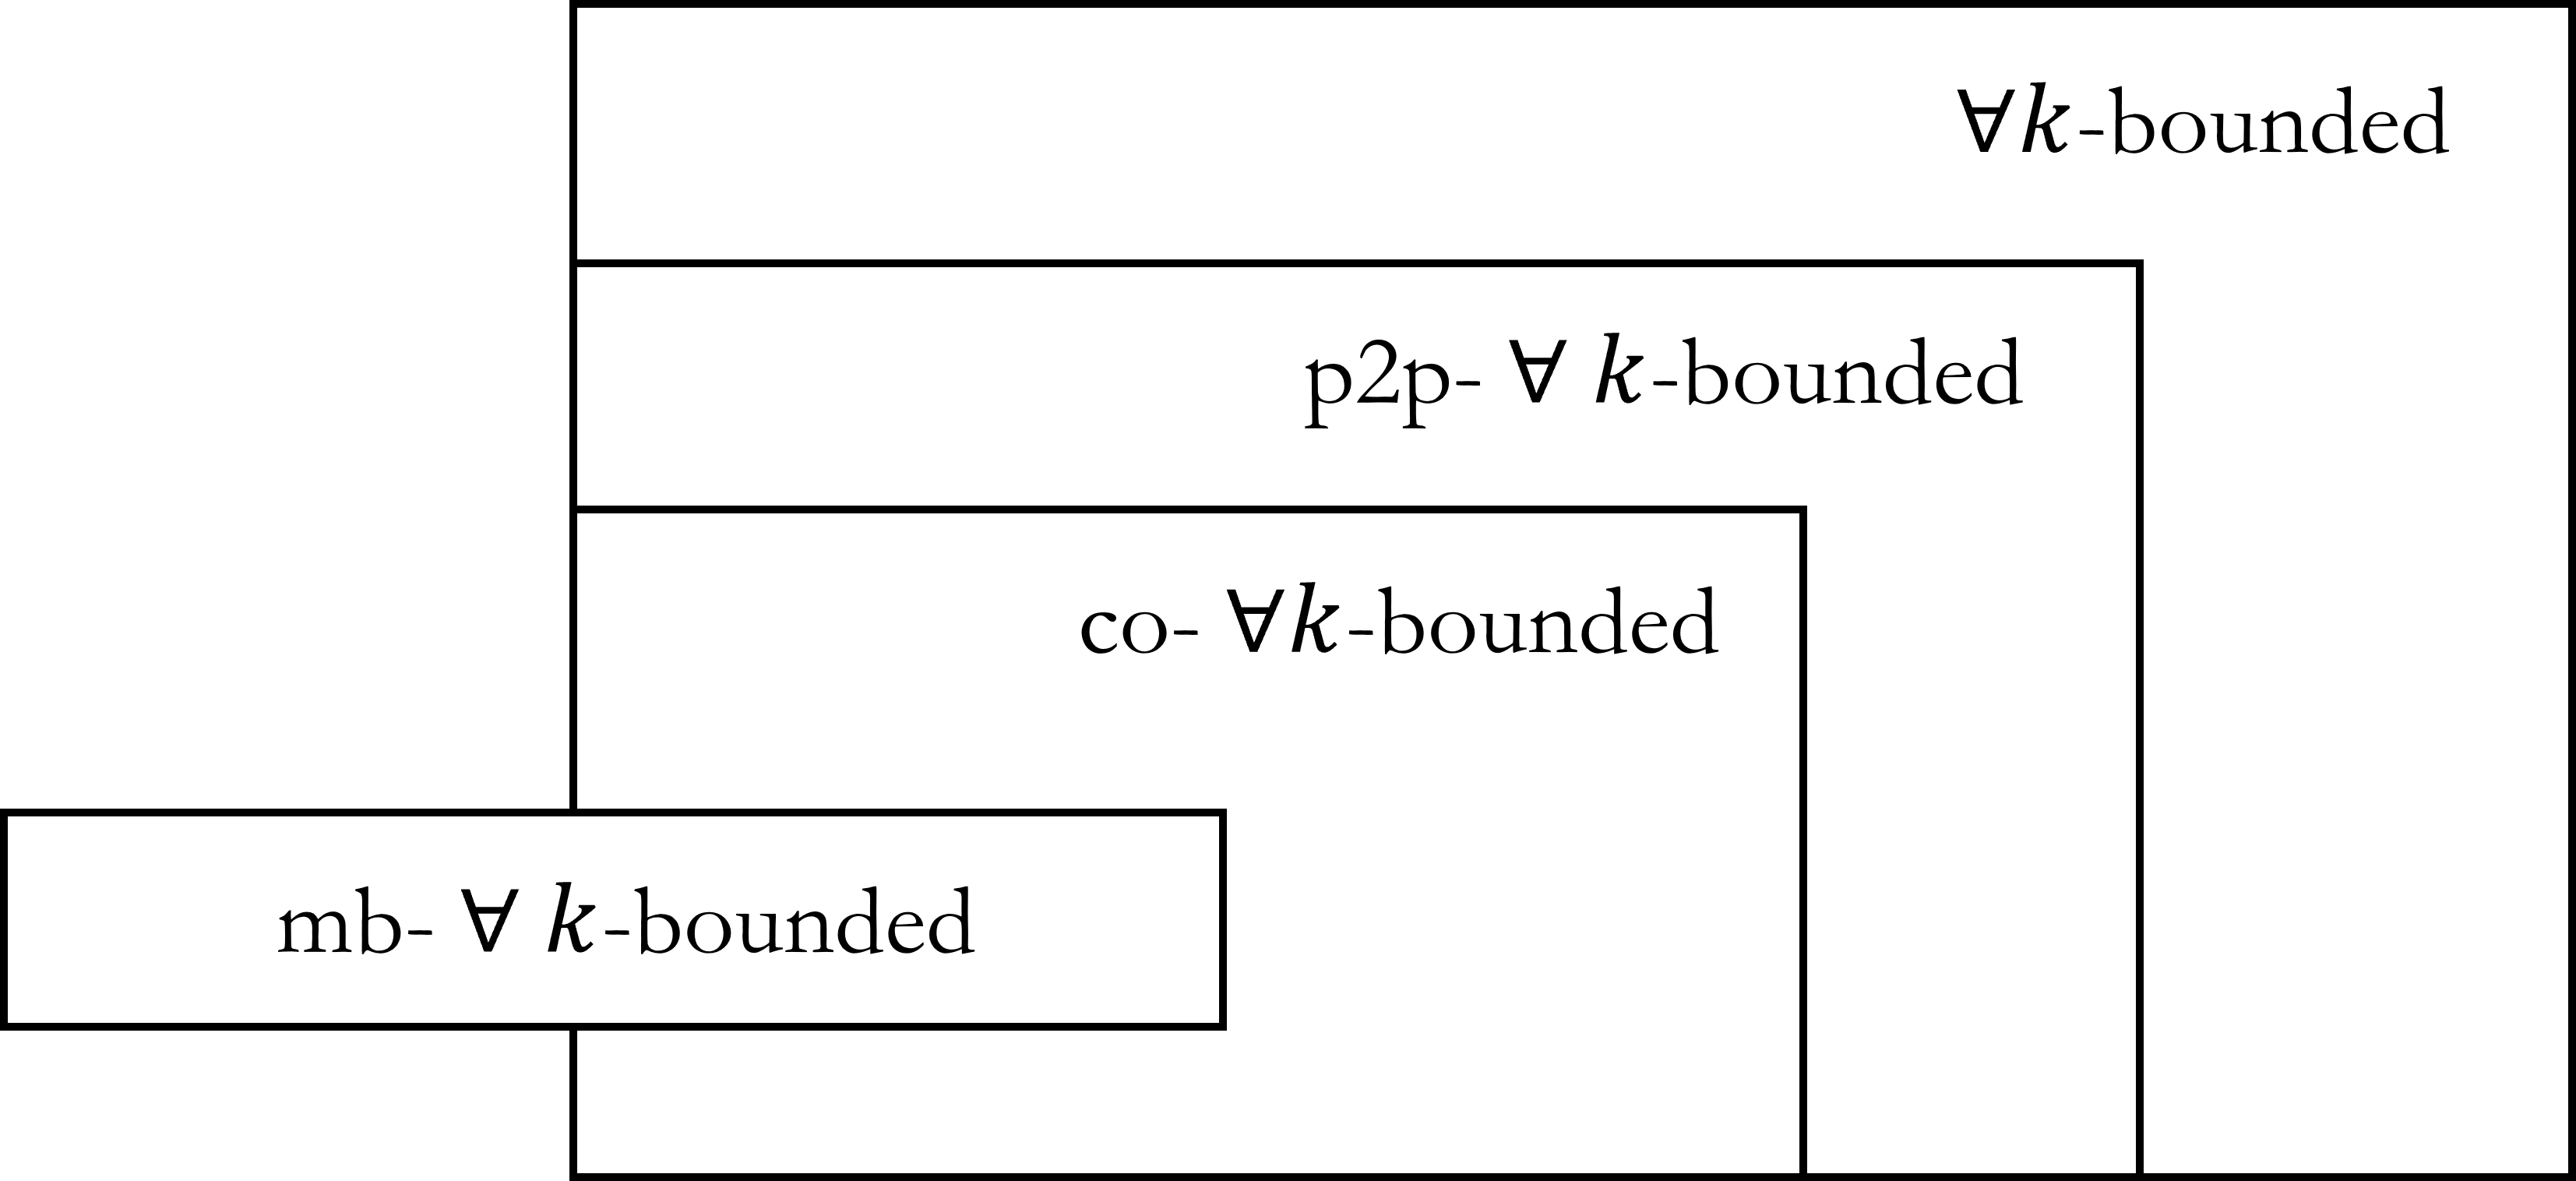
\includegraphics[width=8cm]{uni_k_hierarchy.png}
% 	\caption{The relation between different variants of universally $k$-bounded MSCs, given a $k \in \N$.}
% 	\label{fig:uk_hierarchy}
% \end{figure}

\subsubsection{MSO-definability}

In this section, we will investigate the MSO-definability of all the variants of universally $k$-bounded MSCs that we introduced.

In \cite{DBLP:conf/fossacs/LohreyM02}, it is shown that an MSC $\msc$ is universally $k$-bounded if and only if $\relb \;\subseteq\; \le_\msc$. In other words, $r \relb s \Rightarrow r \le_\msc s$ for any two events $r$ and $s$. This is equivalent to saying that every linearization $\linrel$ of $\msc$ respects the $\relb$ relation, since $\relb \;\subseteq\; \le_\msc \;\subseteq\; \linrel$. We already showed that $\relb$ is MSO-definable. The MSO formula that defines universally $k$-bounded  MSCs can be written as
\[ \asUkformula = \neg \exists r.\exists s.(r \relb s \wedge \neg(r \le_\msc s)) \]
Causally ordered and \pp universally $k$-bounded MSCs are clearly MSO-definable by definition, since we already showed that \pp MSCs, causally ordered MSCs, and universally $k$-bounded MSCs are all MSO-definable. To show MSO-definability of mailbox universally $k$-bounded MSCs we first prove the following property.

\begin{proposition}\label{prop:mb_ukb_alt}
	An MSC $\msc$ is mailbox universally $k$-bounded if and only if $\relb \;\subseteq\; \preceq_\msc$.
\end{proposition}
\begin{proof}
	Consider an MSC $\msc$ and a $k \in \N$.\newline
	($\Leftarrow$) Suppose $\relb \;\subseteq\; \preceq_\msc$. For every mailbox linearization $\mblinrel$ of $\msc$ we have that $\preceq_\msc \;\subseteq\; \mblinrel$. This implies $\relb \;\subseteq\; \mblinrel$, that is to say every mailbox linearization is $k$-bounded.\newline
	($\Rightarrow$) Suppose $\msc$ is a mailbox universally $k$-bounded MSC. By definition, every mailbox linearization $\mblinrel$ of $\msc$ is $k$-bounded, i.e. $\relb \;\subseteq\; \mblinrel$, and we have $\preceq_\msc \;\subseteq\; \mblinrel$, according to the definition of mailbox linearization. Moreover, we also know that $\preceq_\msc \cup \relb$ is acyclic, since $\msc$ is existentially $k$-bounded\footnote{Every mailbox universally $k$-bounded MSC is also a mailbox existentially $k$-bounded MSC by definition.}. Suppose now, by contradiction, that $\relb \;\nsubseteq\; \preceq_\msc$. Thus, there must be at least two events $r$ and $s$ such that $r \relb s$ and $r \npreceq_\msc s$; we also have $s \npreceq_\msc r$ because of the acyclicity of $\preceq_\msc \cup \relb$ (we cannot have the cycle $r \relb s \preceq_\msc r$). Consider a mailbox linearization $\mblinrel$  of $\msc$, such that $s \mblinrel r$. Note that such a mailbox linearization always exists, since $r$ and $s$ are incomparable w.r.t. the partial order $\preceq_\msc$ (i.e. $s \npreceq_\msc r$)\footnote{If two elements $a$ and $b$ of a set are incomparable w.r.t. a partial order $\le$, it is always possible to find a total order of the elements (that respects $\le$) where $a$ comes before $b$, or viceversa.}. This mailbox linearization does not respect $\relb$ (because we have $s \mblinrel r$ and $r \relb s$), so it is not $k$-bounded. This is a contradiction, since we assumed that $\msc$ was a mailbox universally $k$-bounded MSC. It has to be that $\relb \subseteq \preceq_\msc$.
\end{proof}

Using Proposition~\ref{prop:mb_ukb_alt}, we can now easily write the MSO formula that defines mailbox universally $k$-bounded MSCs as
\[ \mbUkformula = \neg \exists r.\exists s.(r \relb s \wedge \neg(r \preceq_\msc s)) \]

\subsubsection{Special treewidth}

All the variants of universally $k$-bounded MSCs that we presented have a bounded special treewidth. This directly follows from the STW-boundness of the existential counterparts, since every universally $k$-bounded MSC is existentially $k$-bounded by definition.
